\paragraph{\glspl{workpiece} und Sortierung}
\begin{itemize}
    \item[REQ-1:] Die \gls{anlage} kann zwischen vier Typen von \glspl{workpiece}n unterscheiden (\gls{workpiece_type}) (2, 3, 4, 5, 6)
    \begin{itemize}
        \item \gls{workpiece_flach} (3)
        \item \gls{workpiece_metall} (4)
        \item \gls{workpiece_bohrung} (5)
        \item \gls{workpiece_hoch} (6)
    \end{itemize}
    \item[REQ-2:] Am Ende des 2.\ \gls{belt}es sollen die \glspl{workpiece} zyklisch in folgender Reihenfolge ankommen (1, 7, 8)
    \begin{enumerate}
        \item \gls{workpiece_metall}
        \item \gls{workpiece_bohrung}
        \item \gls{workpiece_flach}
    \end{enumerate}
    \item[REQ-3:] \glspl{workpiece}, die nicht in die Sortierreihenfolge passen werden in eine der beiden \glspl{rampe} aussortiert (9, 10)
    \item[REQ-4:] Der \gls{durchsatz} an \glspl{workpiece} ist zu optimieren (11)
    \item[REQ-30:] Aussortierung der \glspl{workpiece} soll mit \gls{weiche} funktionieren (41)
    \item[REQ-38:] Aussortierung der \glspl{workpiece} soll mit \gls{ejector} funktionieren (41)
    \item[REQ-39:] Beliebige Kombinationen der \gls{sortierer} an den beiden \glspl{anlage} sollen unterstützt werden. (42)
    \item[REQ-47:] Wenn ein \gls{workpiece_bohrung} oder \gls{workpiece_metall} umgedreht wird, ist es ein \gls{workpiece_hoch}.
\end{itemize}

\paragraph{Kapazität}
\begin{itemize}
    \item[REQ-5:] Bei einer vollen \gls{rampe} wird eine Warnung ausgesandt (12)
    \item[REQ-6:] Wenn die nächste notwendige Aussortierung aufgrund von ausgeschöpfter \glspl{rampe}kapazität
    nicht stattfinden kann, ein Fehler ausgesendet (und somit der Gesamtbetrieb gestoppt) (13)
\end{itemize}

\paragraph{Durchlassablauf}
\begin{itemize}
    \item[REQ-7:] Zuführung von \glspl{workpiece}n erfolgt durch Einlegen von \glspl{workpiece}n am Anfang von \gls{anlage} 1 (14, 15)
    \begin{itemize}
        \item Ein Unterbrechen der \gls{lb_st} signalisiert dem System das Einlegen eines \gls{workpiece}s,
        sodass der Transport dessen beginnen kann.
    \end{itemize}
    \item[REQ-9:] Das System muss mit in beliebigem Abstand eingelegten \glspl{workpiece}n umgehen können(16,17) %TODO Mindestabstand
    \begin{itemize}
        \item Solange der Bereich der ersten Lichtschranke frei ist, muss der Benutzer \glspl{workpiece}
        einlegen können, ohne die Korrektheit der Funktion zu gefährden.
    \end{itemize}
    \item[REQ-14:] Der Abstand von \glspl{workpiece}n auf \gls{belt} 2 muss mindestens 25 cm betragen (18)
    \begin{itemize}
        \item Abstand muss vor der Übergabe sichergestellt werden
    \end{itemize}
    \item[REQ-16:] Auf dem \gls{belt} von \gls{anlage} 2 dürfen sich maximal 2 \glspl{workpiece} befinden (19)
    \item[REQ-18:] Falls sich bei der Übergabe zwischen den beiden \glspl{belt} ein \glspl{workpiece}
    überschlägt, muss der neue \gls{workpiece_type} beachtet werden. (20)
    \begin{itemize}
        \item Der Fall, dass das Teil auf die Seite fällt, sodass es wegrollen könnte, wird ausgeschlossen.
        Wenn sich das \gls{workpiece} überschlägt, ändert sich bei hohen \glspl{workpiece}n der Typ.
    \end{itemize}
    \item[REQ-20:] \glspl{workpiece} dürfen nicht vom \gls{belt} fallen (21)
    \item[REQ-24:] Beim Einlegen eines \glspl{workpiece}s in die \gls{anlage} soll dem \gls{workpiece} eine eindeutige ID zugewiesen werden(28)
    \item[REQ-26:] Wenn sich auf einem \gls{belt} kein \gls{workpiece} befindet, stoppt das \gls{belt}.
    \item[REQ-31:] Wenn ein \gls{workpiece} die \gls{lb_en} von FB2 erreicht,
    sollen Informationen zu diesem \gls{workpiece} auf der Konsole ausgegeben werden (22, 23, 24, 25, 26, 27)
    \begin{itemize}
        \item Zu den Informationen zählen die ID, Typ, Höhe auf \gls{anlage} 1 und \gls{anlage} 2 des \gls{workpiece}es als
        auch ein Hinweis darüber, ob sich das \gls{workpiece} überschlagen hat.
    \end{itemize}
\end{itemize}

\paragraph{Bedienung durch Taster}
\begin{itemize}
    \item[REQ-12:] Bei Betätigung des START-Tasters wechselt die \gls{anlage} in den Betriebszustand (49)
    \item[REQ-15:] Bei Langem Drücken von drei Sekunden des START-Tasters wechselt die \gls{anlage} in den Service-Modus (50)
    \begin{itemize}
        \item Im Service Modus führt die \gls{anlage} Kalibrierung und Selbsttests durch.
        Anforderung hierfür ist, dass die \gls{anlage} im Ruhezustand ist.
    \end{itemize}
    \item[REQ-17:] Bei Betätigung des STOPP-Tasters wechselt die \gls{anlage} in den Ruhezustand (51, 52)
    \begin{itemize}
        \item Dafür müssen bestehende Fehler behoben und quittiert und gegangene Fehler quittiert sein.
        Alles andere führt zu einer Fehlermeldung.
    \end{itemize}
    \item[REQ-21:] Bei Betätigung des RESET-Tasters werden sämtliche Fehler quittiert (53)
    \item[REQ-28:] Wenn die \gls{anlage} durch ESTOPP stillgelegt ist, kann der Betrieb durch Drücken des
    RESET-TASTERs der \gls{anlage}, an dem auch der E-Stopp-Schalter gedrückt wurde, fortgesetzt werden (56)
    \begin{itemize}
        \item Bedingung dafür: Keine ESTOPP-Schalter sind gedrückt
    \end{itemize}
    \item[REQ-40:] Im Service Modus führt die \gls{anlage} beispielsweise Kalibrierung und Selbsttests durch (50)
    \begin{itemize}
        \item Aus dem Anforderungsdokument geht dies nicht eindeutig hervor, dies muss in zukünftig spezifiziert werden.
    \end{itemize}
    \item[REQ-41:] Bei Betätigung des ESTOPP-Schalters werden beide \glspl{anlage} angehalten (54, 55)
    \item[REQ-42:] Dem Benutzer werden Hinweise über die Benutzung der \gls{anlage} mithilfe der LEDs an der Tastatern gegeben
    \begin{itemize}
        \item Im Betriebszustand ist die LED am Start-Taster an, im Ruhezustand die LED am Stopptaster.
        Bei einem gegangenen oder bestehenden Fehler ist die LED am RESET-Taster an.
    \end{itemize}
\end{itemize}

\paragraph{Zustandsanzeigen}
\begin{itemize}
    \item[REQ-10:] Im Betriebszustand leuchtet die \gls{ampel} grün dauerhaft (59)
    \item[REQ-11:] Im Service-Mode blinkt die \gls{ampel} grün (60)
    \item[REQ-13:] Bei Warnungen blinkt die \gls{ampel} gelb (61)
    \begin{itemize}
        \item Eine Warnung ist, dass die \gls{rampe} an der \gls{anlage} voll ist.
    \end{itemize}
    \item[REQ-19:] Wenn keine Warnungen vorliegen ist die gelbe \gls{ampelled} aus (61)
    \item[REQ-37:] Die rote \gls{ampelled} signalisiert die Fehlerzustände wie folgt (73, 74, 75, 76):
    \begin{itemize}
        \item Anstehend unquittiert wird durch schnelles Blinken (1 Hz) signalisiert (74).
        Anstehend quittiert wird durch dauerhaftes Leuchten(75) signalisiert.
        Gegangen unquittiert wird durch langsames Blinken (0,5 Hz) signalisiert (z.B.\ wenn ein
        \gls{workpiece} an einer \gls{weiche} zu langsam in die \gls{rampe} geschoben wurde) (76).
        Steht kein Fehler an, ist die Leuchte aus (73).
    \end{itemize}
    \item[REQ-45:] Im Ruhezustand leuchtet die \gls{ampel} dauerhaft gelb
\end{itemize}

\paragraph{\gls{weiche}}
\begin{itemize}
    \item[REQ-23:] Verklemmen der \gls{weiche} soll überwacht werden (37)
    \begin{itemize}
        \item Ein \gls{workpiece} ist verklemmt, wenn das \gls{workpiece}, abzüglich der Toleranz von 50 Prozent
        der durchschnittlichen Aussortierzeit, länger als erwartet braucht, um in der \gls{rampe} anzukommen.
        Daraufhin wird eine Warnung ausgesendet, bis das Teil in der Rampe ankommt.
    \end{itemize}
    \item[REQ-27:] Die \gls{weiche} darf nicht länger als 'x' auf offen stehen (35, 36)
    \begin{itemize}
        \item Bei minutenlangen Stromfluss wird die \gls{weiche} beschädigt.
    \end{itemize}
\end{itemize}

\paragraph{Embedded Recorder}
\begin{itemize}
    \item[REQ-25:] Es soll eine 'record'-Funktion bereitgestellt werden, mit der ein Benutzer das gesamte
    Ereignisprotokoll der \gls{anlage} aufzeichnen kann (90)
    \item[REQ-29:] Die von der 'record'-Funktion vorgenommene Aufzeichnung soll menschenlesbar sein (91)
    \item[REQ-33:] Es soll eine 'replay'-Funktion bereitgestellt werden, mit der ein
    Benutzer eine zuvor aufgezeichnete Ereignissequenz abspielen lassen kann (93, 94)
    \item[REQ-34:] Ereignissequenzen sollen per Hand angefertigt werden können (95, 96)
\end{itemize}

\paragraph{Höhenmessung}
\begin{itemize}
    \item[REQ-32:] Höhenmessung muss Kippung des Lasers mit einbeziehen (43, 44)
\end{itemize}

\paragraph{Fehlerumgang}
\begin{itemize}
    \item[REQ-35:] Nach Behebung eines Fehlers soll der Normalbetrieb fortgesetzt werden. (45, 46)
    \begin{itemize}
        \item Nach Möglichkeit sollen die \glspl{belt} nicht geräumt werden.
    \end{itemize}
    \item[REQ-43:] In den Zuständen 'bestehend\_unquittiert' und 'bestehend\_quittiert' bleiben die
    \glspl{belt} beider \glspl{anlage} stehen und den Aussortiermechanismen wird der Strom abgestellt
    \begin{itemize}
        \item Die Fehleranzeige über die \gls{ampel} ist in REQ-37: spezifiziert
    \end{itemize}
    \item[REQ-36:] Fehlerzustand soll wie in Abbildung~\ref{fig:stm-fehlerzustand} beschrieben sein. (65, 66, 67, 69, 70)
    \item[REQ-46:] Der globale Fehlerzustand wird wie folgt festgelegt
    \begin{itemize}
        \item Der aktuell bestehende Fehler mit der höchsten Priorität entspricht dem Fehlerzustand der gesamten \gls{anlage}.
        Die Fehlerzustände sind der folgenden Liste nach priorisiert: 1.\ Anstehend unquittiert
        2.\ Anstehend quittiert 3\ Gegangen unquittiert 4.\ OK
    \end{itemize}
\end{itemize}

\begin{figure}[h]
    \centering
    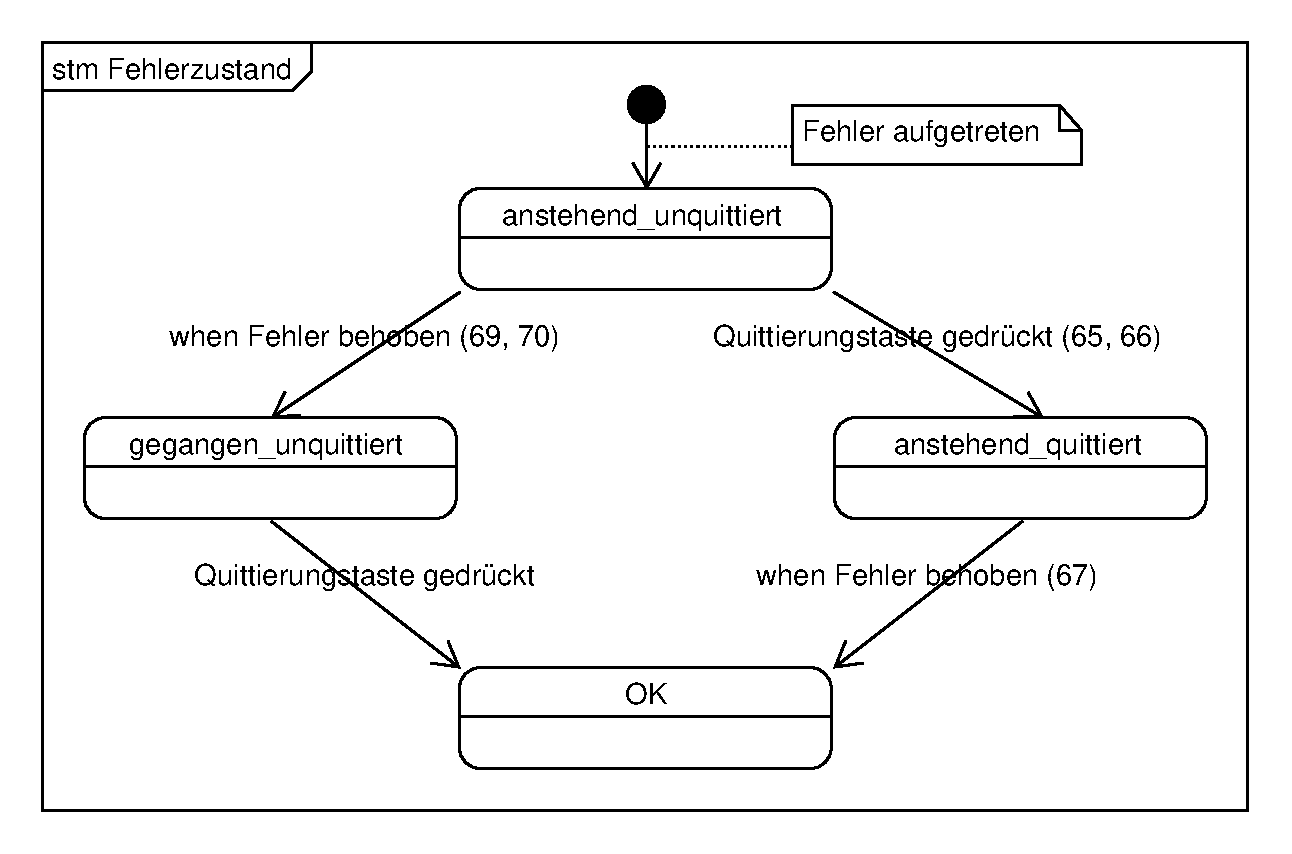
\includegraphics[scale=0.5]{../out/diagrams/stage1/req-fehlerzustand}
    \caption{REQ-36 Visualisierung des Fehlerzustandes eines einzelnen Fehlers}
    \label{fig:stm-fehlerzustand}
\end{figure}
